\chapter[Mental Models of Password Managers]{Mental Models of Password Managers}\label{chap:mental_models_pwm}
%lingo: prospective users.
An important spillover of our previous exploration is that password managers are more likely adopted the longer people had struggled with juggling passwords: Older participants in the third personality study (Section \ref{sec:personality:study3}) were more likely to use a \gls{PWM}. We have already corroborated market surveys that indicate a generally low adoption rate of password management software. As discussed in Sections \ref{sec:rw:user-behavior} and \ref{sec:rw:pwm_generators}, it has been hypothesized that users do not fully trust third parties with their credentials, so there seems to be an urge to stay in charge. Consequently, most users still try to memorize their passwords. On the other hand, password managers do provide many usability and security benefits, but why do users fail to see them? To this end, we see a lack of understanding about how users make sense of password managers. Our goal was to understand users' mental models of password managers first and then identify opportunities to improve them, which could increase adoption rates. 
%RQs
We thus aimed to answer the following research questions: 
\textbf{(1)} How do users think a password manager works? 
\textbf{(2)} How does adopting a password manager change user attitudes and behaviors?


To answer these questions, Martin Prinz and I explored attitudes and understandings in semi-structured qualitative user interviews. To get a more complete picture, we interviewed both people who already use a \gls{PWM} and also people who prefer other coping strategies. Parts of the outcome of this investigation have been published as an extended abstract at SOUPS 2017 \cite{Prinz2017MentalModel}.

\section{Background and Context}
%%%
% technical side
%%%

% PWM have existed since xyz. -- not possible to point a specific origin. 
Password managers can be either built into web browsers or act as a standalone solution that is independent of the password's purpose. Dedicated password managers have existed since the mid to late 1990s. Web Confidential\footurl{http://www.web-confidential.com/}{16.02.2018} was probably one of the first programs to facilitate password management, when it first surfaced in 1998. However, which of the browsers was first to add password storage capabilities cannot be easily traced back, but all major browsers added this feature in the early 2000s. Given the long history of supporting authentication with software tools, adoption of password managers is still at only 12\% \cite{Olmstead2017AmerciansCybersecurity}. Even security experts disagree on the specific security benefits of different implementations\footurl{https://www.wired.com/2015/07/websites-please-stop-blocking-password-managers-2015/}{16.02.2018}. If the auto-fill feature is enabled, this can be used to create digital footprints for individuals\footurl{https://freedom-to-tinker.com/2017/12/27/no-boundaries-for-user-identities-web-trackers-exploit-browser-login-managers/}{16.02.2018}. Nevertheless, similar attack vectors could easily target regular password entry, and are not limited to auto-fill. 

% different system architectures: built into browser, local software (dedicated programm and/or browser extension), distributed storage.
There are different service architectures for handling passwords: \textit{offline} password managers keep a database of encrypted passwords locally on the user's machine, while \textit{online} managers provide more mobility because passwords are held on a server or a distributed storage solution \cite{McCarney2012Tapas}. \textit{KeePass} and \textit{Password Safe} are notable representatives for the offline storage paradigm, while the cloud-based approach is dominated by third-party solutions like \textit{LastPass}, \textit{1Password}, and \textit{Dashlane}. Browser vendors have also transitioned to store passwords in the cloud, e.g. Apple Keychain for Safari, or Google Smartlock for Chrome. On the one hand, this provides consistent user experiences across multiple devices. On the other hand, such architectures create lock-in effects and dependencies. Thus, online password managers typically provide browser-extensions to automatically fill username and password fields. This way, similar experiences are achievable by third party tools. 

% pwms are not universally accepted as the best solution.
% some websites block password managers (by disabling the ``paste'' event on their login form), because under some circumstances password managers can be used to track users. 

%%%
% user side:
%%%
% academic

% briefly summarize experiments focused around mental models of password managers
\paragraph{Mental Models} 
%motivation
Norman suggests that exploring mental models provides predictive and explanatory power for understanding an interaction \cite{Norman1982ObservationsMentalModels}. Volkamer and Renaud meticulously described different aspects and definitions of mental models, which are too elaborate to discuss in this work \cite{Volkamer2013MentalModels}. As a takeaway, a mental model describes a user's sense-making of any system they interact with. Volkamer and Renaud highlight that mental models are not necessarily static, but can be shaped with different cues to internal feedback loops (see Figure \ref{fig:mm_pwm:mental-model-volkamer}). For our purposes, we use a simpler definition provided by Young: Mental models are ``collections of the root reasons why a person is doing something'' and ``represent what a person is trying to accomplish in larger context, no matter which tools are used''  \cite[p.11]{Young2008}. In our case, they describe the reasons for (not) using a password manager, as explained by current actions to cope with authentication tasks. 

\begin{figure}
	\centering
	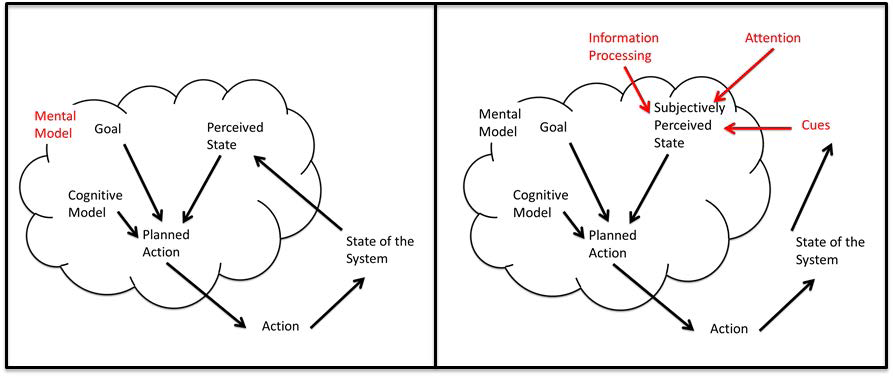
\includegraphics[width=\linewidth]{mm_pwm/MentalModels-volkamer}
	\caption{\label{fig:mm_pwm:mental-model-volkamer} Volkamer and Renaud see the formation of mental models as loop involving different plans, perceptions, system structures, and actions. Image from \cite{Volkamer2013MentalModels}}
\end{figure}
% what is different now? quant --> qual
In chapter \ref{chap:pasdjo}, we took a quantitative approach to elicit data on the mental models. This was useful because we tried to understand \textit{what} contributed to password strength perceptions and by \textit{how much}. For password managers, related work on usage motivation is scarce, thus we strove to answer \textit{why} users perform certain actions and \textit{how} these could be supported by a password manager. Therefore, qualitative methods were more useful. 
% how is this qual data elicited?
Eliciting such data to understand mental models, Bravo-Lillo \etal relied on open-ended one-on-one interviews both with advanced and novice user groups \cite{BravoLillo2011WarningsMentalModel}. They highlight the usefulness of this approach to understand thought processes. Kang \etal relied on \textit{drawing tasks} to elicit additional data \cite{Kang2015MentalModelsDrawing}. Participants were asked to sketch what they thought happens to their personal data when they interact with different online services. During sketching, a \textit{concurrent think-aloud protocol} was used to avoid misunderstandings. Once the data has been collected, Young suggests the \textit{affinity diagramming} method to derive themes and identify opportunities for supporting tasks \cite{Young2008}. In this research project, we combined interviewing, drawing tasks, and affinity diagramming. 

\section{User Interviews}
Our main objective was to understand how users make sense of password support tools, in particular password managers. This would allow us to explore solutions that fit user expectations better.  

\subsection{Method and Protocol}
Focusing on attitudes and mental models requires a qualitative study method. We chose to conduct semi-structured, open-ended interviews. The sessions started with a thorough briefing about the study purpose and asking for permission to audio-record the conversation. The main questions were \textbf{(1)} \textit{Why do you need passwords?} and \textbf{(2)} \textit{What is your strategy to manage multiple accounts?}. From there, the study followed a more fine-grained follow-up questions to investigate the specifics of these two aspects. Moreover, Bravo-Lillo \etal showed the benefits of drawing tasks to find structural patterns in beliefs \cite{BravoLillo2011WarningsMentalModel}, so we also asked participants to \textbf{(3)} \textit{sketch how a password manager works}. This required that participants were aware of \glspl{PWM}. If they were not, they were told that it is a ``piece of software that stores a user's password'', which was expected to be vague enough to explore participants' expectations of this kind of software. The interviews took between five and 16 minutes. 

\subsubsection{Recruitment and Sample}
We first approached random passers-by on a popular street in Munich to obtain a diverse sample of participants. Six interviewees were recruited this way. However, these first six interviews showed that participants were unable to provide sufficient detail in answers to allow thorough analysis. Thus, we changed the recruiting method and approached employees of a design agency with which we had collaborated in the past. We also knew that the agency's policy required employees to utilize password managers. Moreover, the user group was more likely capable of visually expressing mental constructs, allowing for the envisioned analyses. Eight additional participants were interviewed in this sample, giving a total of N=14. They worked as experience designers and concept developers, and did not have formal training in computer science or engineering. The age of all interviewees ranged from 20 to 41. \todo{listen to recordings and determine gender distribution (CD in Munich)}. 

None of the interviewees in the first group had used a password manager before, so we call this participant group the \textit{novices}. Since the \gls{PWM} was part of the company policy, all interviewees in the second group had used one before, so we call them the \textit{actives}. The separation allowed us to detect a shift of expectations before and after adopting a password manager. 

\subsubsection{Method Limitations}
The recruiting and sampling methods are inherently limited. The novice user group was asked at a public spot, so it was difficult to provide enough contextual information and minimize distraction. On the plus side, we achieved diversity and the face-to-face set-up reassures trust, because it was clear that none of the information they gave us was going to be used to access their online accounts. 5 of 6 \textit{novices} were unable to describe what a password manager was, before we gave them the above definition. Thus, their decision to refrain from using a \gls{PWM} was not made actively, but rather results from the lack of awareness. This limits the analysis of attitudes and self-reported behavior. Finally, the second user group has a homogeneous background: design and communication. All these limitations demand that the results not be generalized to a larger population. Instead, they should be seen as rough trends that help understand a first set of underlying mental models, rather than the entire spectrum thereof.

\subsection{Data Analysis and Results}
% analysis approach
Young proposed a design strategy to translate qualitative data into mental models \cite{Young2008}. The method is based on \textit{affinity diagramming}. The resulting clusters and themes from the diagram are then mapped to a hierarchical structure that consists of Mental Spaces, Task Towers, Tasks, and Particular Tasks. Here, we focused on those Mental Spaces and Task Towers that involve password managers. Table \ref{tab:mm_pwm:mental-model-table} shows the resulting model in this format. In the following, we report the results that notably contributed to the formation of the model, which is described in Section \ref{ref:mm_pwm:mm-description}.

\begin{table}[htpb]
\def\arraystretch{1.05}% 
\begin{threeparttable}
\begin{tabular} {l|l|l}
\textbf{Mental Space} & \textbf{Task Tower} & \textbf{Tasks} \\ \hline\hline
Creation \& Selection
& Influential Factors & Personal \& Historical \\ 
& & Policies \& Rules \\
& & Algorithmic Strategies \\
& & Account Context \\
& & Memorization \\ \cline{2-3}
& Support Tools & Generate \& Memorize \\
& & Use given Password \\
& & Generate \& Digitally Store \\ \cline{2-3}
& Personal Algorithms & Passphrases \\
& & Reuse Word Blocks \\
& & Base-Password with Modifications \\
& & Website Influence \\
& & Use Reduced Alphabet \\\cline{2-3}
& Handle Failures & Trial and Error \\ 
& & Lookup Password \\
& & Show Entered Password in Plain Text\\
& & Reset Password \\ \hline 
Log-In 	& Manual Tasks 	& Copy \& Paste password \\
	 	& 		 	& Lookup hints and cues \\ 
	 	& 		 	& Recall from memory \\ 
\cline{2-3}
		& Simplify 	& Stay logged-in \\ 
		& 			& Cross-device support \\ 
		& 			& Autofill forms \\ 
		& 			& Rely on manager \\ \hline
Organize and Commit & Share Passwords & Secure sharing with colleagues or friends \\
		&			& Write down password \\
		&			& Reset after sharing\\ \cline{2-3}
		& Use Aid & Password Manager \\
		& 		 	& Word/Digital Document \\ 
		& 		 	& Handwritten Notes \\  \cline{2-3}
		& Memorize Passwords & Algorithmic \\ 
		&			& Website Cues \\
		& & Mental Drawer \\
		& & Base Password and Modifications \\ \cline{2-3}
		& Protect Passwords & Modify Passwords \\
		& 			& Unlock access with Master Password\\
		&			& Hide or Encrypt File/Notes \\ \cline{2-3}
		& Automation & Reset Multiple Passwords\\
		&  			& Autosave Credentials \\ 
		&			& Autofill Username and Password \\
		&			& Warnings when websites are compromised \\\cline{2-3}
		& Build Password Categories & Security \\ 
		&			& Importance \\
		&			& Frequency \\
		&			& Policies \& Rules \\
		&			& Mental Drawer \\ \hline

\end{tabular}
\end{threeparttable}
\caption{\label{tab:mm_pwm:mental-model-table}
	Mental Model of Authentication and Password Management, adapted from Martin Prinz \cite{Prinz2017Thesis}}
\end{table}% \ref{tab:mm_pwm:mental-model-table} %
%\begin{figure}
%	\centering
%	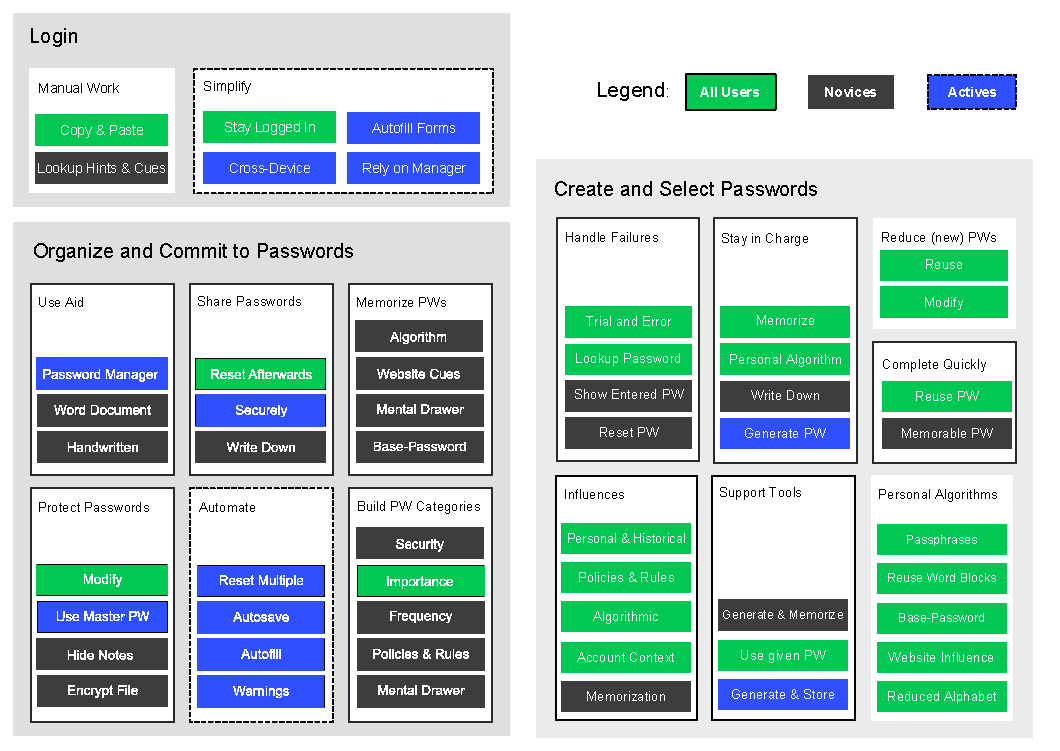
\includegraphics[width=\linewidth]{mm_pwm/mental-model-diagram}
%	\caption{\label{fig:mm_pwm:mental-model-diagram} Mental model diagram}
%\end{figure}


\subsubsection{Selection and Coping Strategies}
All interviewees reuse passwords to cope with the multitude of accounts. Participants often developed coping strategies without deliberation: they were unaware of how they cope with passwords until we specifically requested more details. Only then did they reflect and realize how they behave. One such revelation was that they categorize passwords in different ways. For instance, the context in which they created an account, e.g. the URL or policy of the corresponding website, was factored into passwords and facilitated the decision-making process which password to choose from their portfolio (see Figure \ref{fig:mm_pwm:creation-strategies} A). Similarly, the perceived importance led to distinct categories, although the interviewees had not realized this. Participants generally tried to justify their ``insecure'' behavior. Beside memory burden of new secrets, time pressure was mentioned as reason for password reuse. 

Furthermore, we also heard an interesting, deliberate strategy that seldom appears in the literature: two participants mentioned memorizing a list, or a list of letters that are then transformed into a new, quasi-unique password. This method is comparable to the Diceware technique (details in Section \ref{sec:rw:passphrases}). Instead of rolling a dice to generate a random number by which to look up a word from a list, those participants algorithmically select the order of words/letters based on contextual cues (see Figure \ref{fig:mm_pwm:creation-strategies} B and C). Another participant said to have memorized a randomly generated password and reusing it many times. 

We also inquired situations when their strategies failed. The primary problem of having a multitude of accounts was the correct \textit{combination} of user-name and password, which is a common pitfall of knowledge-based authentication \cite{Stobert2014PasswordLifeCycle}. Not only did they forget passwords, but also user names, which is just as severe because web sites generally do not inform users which was the error source to thwart attacks. Participants reportedly use a trial-and-error approach to go through their portfolio and ultimately use self-serviced password resets as a convenient solution. Interviewees expected that websites offer this kind of fallback scheme, because two of them do this on a regular basis. 

\subsubsection{Password Manager Impact}
Overall, the \textit{novices} and \textit{actives} did not behave differently in their selection and coping strategies at first sight. However, we found that \textit{actives} did in fact change some habits when they had started using a password manager. First, although they were initially exposed to \glspl{PWM} at work, \textit{actives} started using them in private shortly afterwards. This interaction and experience with the tool led to their migrating passwords into the manager step by step. One participant mentioned that it helps him stay organized where there was ``chaos'' before (see Figure \ref{fig:mm_pwm:creation-strategies} C). Others were somewhat ashamed of their weak practices before using this kind of software. 
Password sharing with other users was the central advantage for four interviewees, especially at work. It facilitates secure collaboration with colleagues and clients. Participants do not memorize these passwords, because they often use built-in password generators. They realized that shared passwords are short-lived because colleagues leave or contracts with clients end, upon which passwords are invalidated. One interviewee fully embraced generated passwords even for private purposes and only memorizes his master password. Interestingly, however, for their most important accounts, most \textit{actives} kept on manually crafting passwords and refrained from putting them into the \gls{PWM}. Having used the tool and become aware of their own weak behavior in the past, they had gained confidence in selecting stronger passwords. This gain of mastery left them with a positive experience of password managers. As a contrast, \textit{novices} were all comfortable with how they managed their passwords and did not show that sense of insecurity.

\begin{figure}
\centering
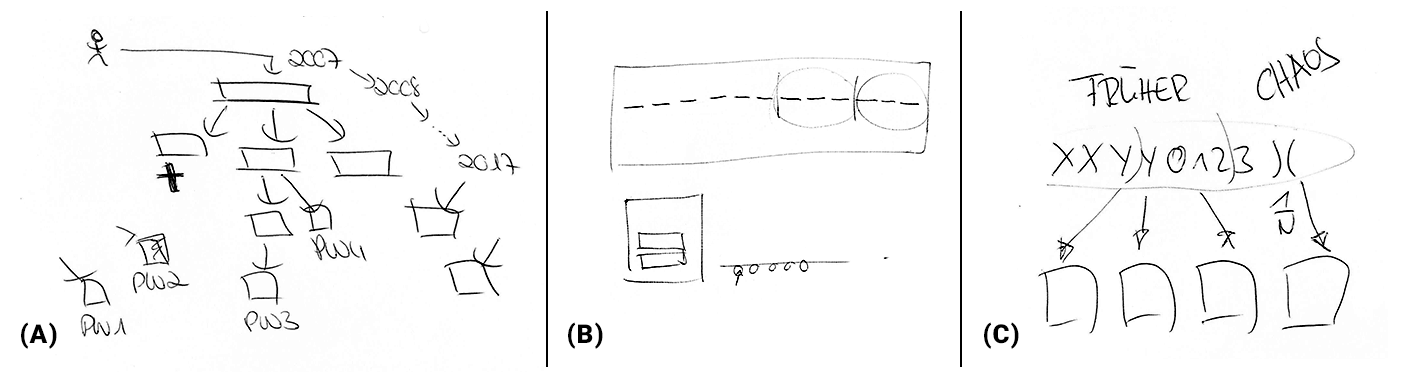
\includegraphics[width=0.9\linewidth]{mm_pwm/f_creation_sketch}
\caption{\label{fig:mm_pwm:creation-strategies}	Participants were asked to visualize their methods to create passwords, if they had a specific strategy. (A) participant who categorizes and remembers passwords by the time they were created (context factors). (B) participant uses words and cued positions to recall the constellation. (C) participant who uses a fixed set of characters and algorithm to ``calculate'' the correct constellation.}
\end{figure}

\subsubsection{Drawing Tasks}
Participants were asked to sketch their thoughts whenever this was appropriate. We encouraged them to sketch as much as possible. All participants mentioned that it was challenging to communicate their understanding this way. Already for basic functionality and purpose of passwords, we asked to create sketches. This task was still relatively easy for all interviewees. Padlocks and keys were two of the most commonly drawn elements. It also helped to communicate individual elaborate selection strategies (see Figure \ref{fig:mm_pwm:creation-strategies}). However, the difficulty rapidly changed for the workings of a password manager.
Here, especially \textit{novices} struggled with the task and could not proceed without further explanation, and their drawings were more vague than those of \textit{actives}. However, the latter is probably due to the different professional background and expertise in creating concepts. The drawn elements and metaphors differed among the two groups: 
\paragraph{Novices} had a vague model of how such a password manager might work and found it especially difficult to sketch this. The benefits and system architecture of the software were unclear to them. One interesting drawing depicted a password manager as a virtual ``brain'' that acts as a central hub to make the user's life easier (Figure \ref{fig:mm_pwm:f_novice_sketch} B). Another participant, who reportedly used a Word document to keep track of his accounts, imagined a password manager to behave the same way (Figure \ref{fig:mm_pwm:f_novice_sketch} C). The only expected difference would be that accessing the list of passwords would be protected by a password, which is indicated by the keyhole and an arrow that points to it. This represents \textit{novices'} understanding on a more general level, as they explained a password manager as a special way to manage a \textit{secure list of passwords} that helps find the right ones. Five said that it facilitates logins by allowing them to \textbf{copy-and-paste} passwords from the manager into the webpage. 
\begin{figure}
	\centering
	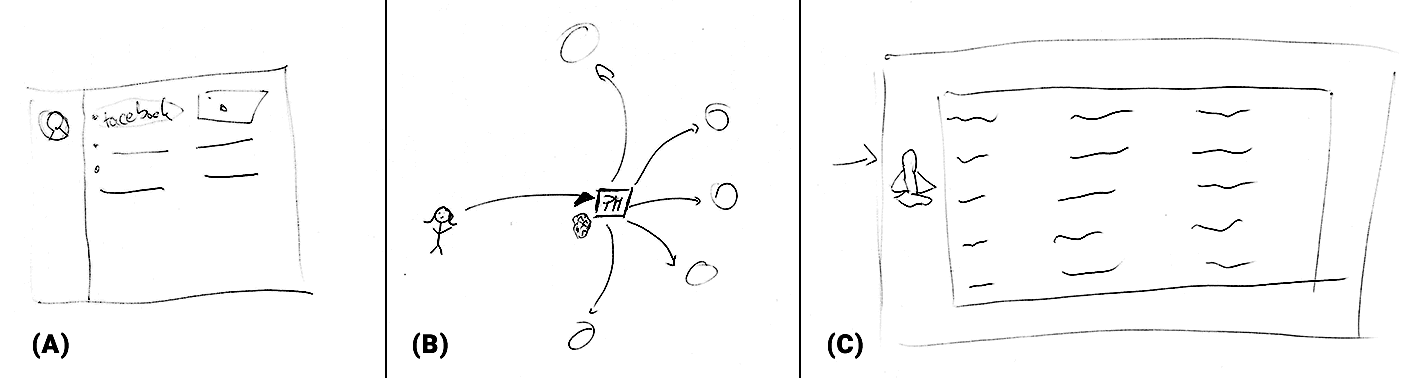
\includegraphics[width=0.9\linewidth]{mm_pwm/f_novice_sketch}
	\caption{\label{fig:mm_pwm:f_novice_sketch}	Drawings to the question ``What does a password manager do, and how?'' from three \textit{novice} users. (A) only shows a profile on facebook. (B) emphasizes that the PWM is a central hub and acts as the user's ``brain'' for different entities. (C) shows a table-like structure that holds all username-password tuples.}
\end{figure}

\paragraph{Actives} Since all active users were also visual communicators, it was somewhat easier for them to sketch the workings of a password manager. They clearly focused on the interaction between users and the system and highlighted the benefits in their drawings. Having experienced the advantages, they strove to convey these visually and came up with more details (cf. Figure \ref{fig:mm_pwm:f_actives_sketch1}). Instead of a password-table, we can see workflows that show the interplay between user, database and website. Common components are UI elements like input fields
or buttons that link to other screens or entities. Only one interviewee from the \textit{active} group refrained from UI elements and instead sketched a flow-chart. 
\begin{figure}
	\centering
	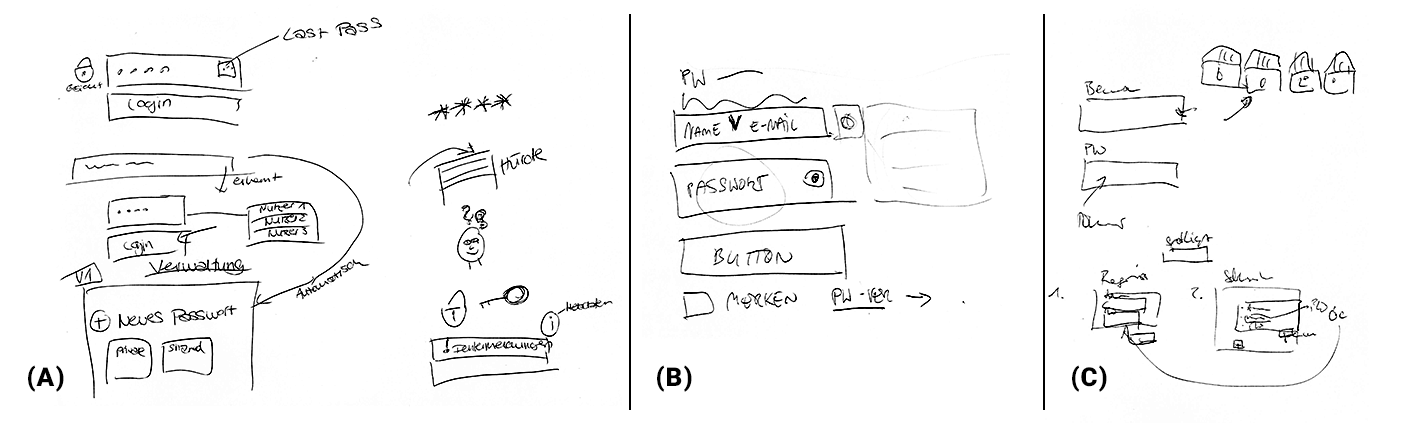
\includegraphics[width=0.9\linewidth]{mm_pwm/f_users_sketch1}
	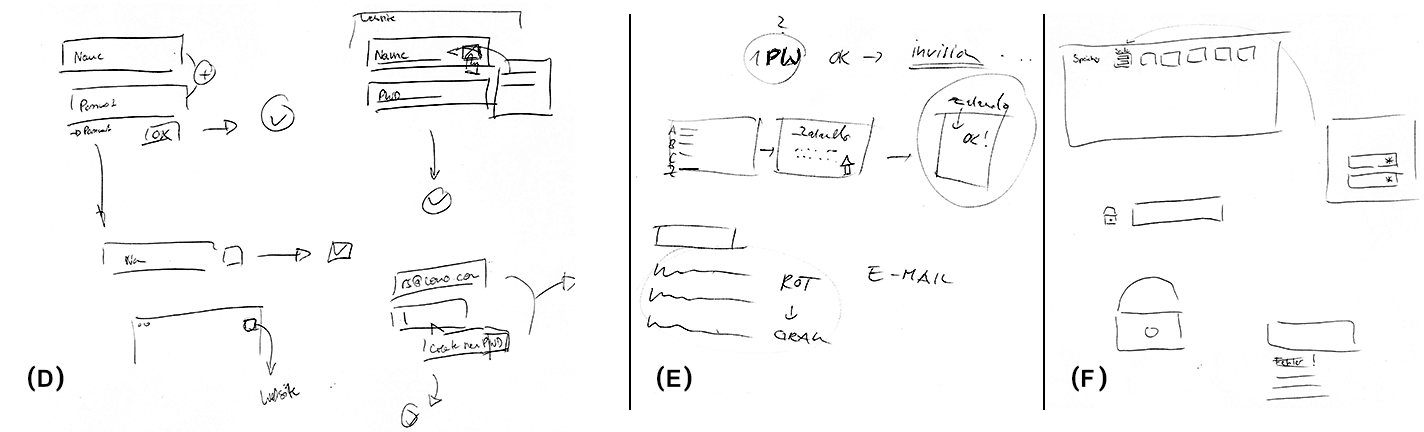
\includegraphics[width=0.9\linewidth]{mm_pwm/f_users_sketch4}
	\caption{\label{fig:mm_pwm:f_actives_sketch1} Drawings to the question ``What does a password manager do, and how?'' from six \textit{active} users. Common components are UI elements that link to other entities, therefore the interplay between user, PWM and website is clearer.}
\end{figure}

\section{Mental Model}\label{ref:mm_pwm:mm-description}
From the behavioral, attitudinal, and experiential data, we created a mental model schema in the style of Young \cite{Young2008}. We tried to stay close to the data as possible, but a few points are enhanced by knowledge from related work. We briefly elaborate on the mental spaces to allow the reader to delve into task-towers and tasks. 

\paragraph{Password Creation and Selection}
First, users have a variety of particular needs when they are challenged to create a password. This task tower describes both the constraints, prior experiences and strategies to accomplish the task. Our participants often mentioned highly individual selection strategies that allow for both secure and memorable secrets. From a support tool, they expected guidance and feedback. Password generators that simplify this task can aid here. 

\paragraph{Log In}
Most prominently, authentication still involves \textit{both} manual and automatic tasks. Interviewees expected to copy and paste passwords from the manager to their browser, or at least provide a way to retrieve password hints.  On the other hand, participants expected that support tools are deeply integrated into the browser by automatically filling password fields in a highly reliable manner. If possible, the solution should work across multiple devices. 

\paragraph{Organize and Commit}
The third mental space resembles the ``Commit to password'' and ``Live with password'' stages of the Password Life Cycle \cite{Stobert2014PasswordLifeCycle}. Each participant mentioned some way of organization strategy that allowed them to live without password managers to some degree. However, these were not always deliberate choices, but rather have formed over the years. Especially \textit{novice} users made sense of password managers by their capability of protecting passwords, i.e. encrypting a list of passwords rather than just storing them in a Word document. \textit{Active} users were already aware of the sharing capabilities and appreciate a simple process to reset passwords when they need to be invalidated for security reasons.

\section{Opportunities and Challenges}
Having fine-grained insights into the mental models of password authentication sub-tasks lets us explore novel ways to support users in many challenges. In the following, we highlight key opportunities for future work on password managers and password support in general. 

\subsection{Leveraging and improving novices' mental models}
There were two important preconceptions about password mangers on the \textit{novices} side: simple password lists and copy-paste interactions. Future password managers can leverage these models to persuasively communicate functionality. The value proposition should thus ensure that potential users understand that PWMs are \textit{not only} a secure list of user-names and passwords, but also help them \textit{select} passwords -- a benefit that \textit{actives} had realized in retrospect. The \textit{password list} metaphor is also useful to communicate automation features: explicitly showing new users that they do not have to search through the list, nor copy and paste passwords from the list to the website might help them understand the simplicity of the interaction paradigm. This can happen during an onboarding user journey, e.g. with an image showing the steps saved by the PWM (cf. Figure \ref{fig:mm_pwm:pwm-goms-comparison}).

\begin{figure}%TODO could make this a little bit nicer. 
	\centering
	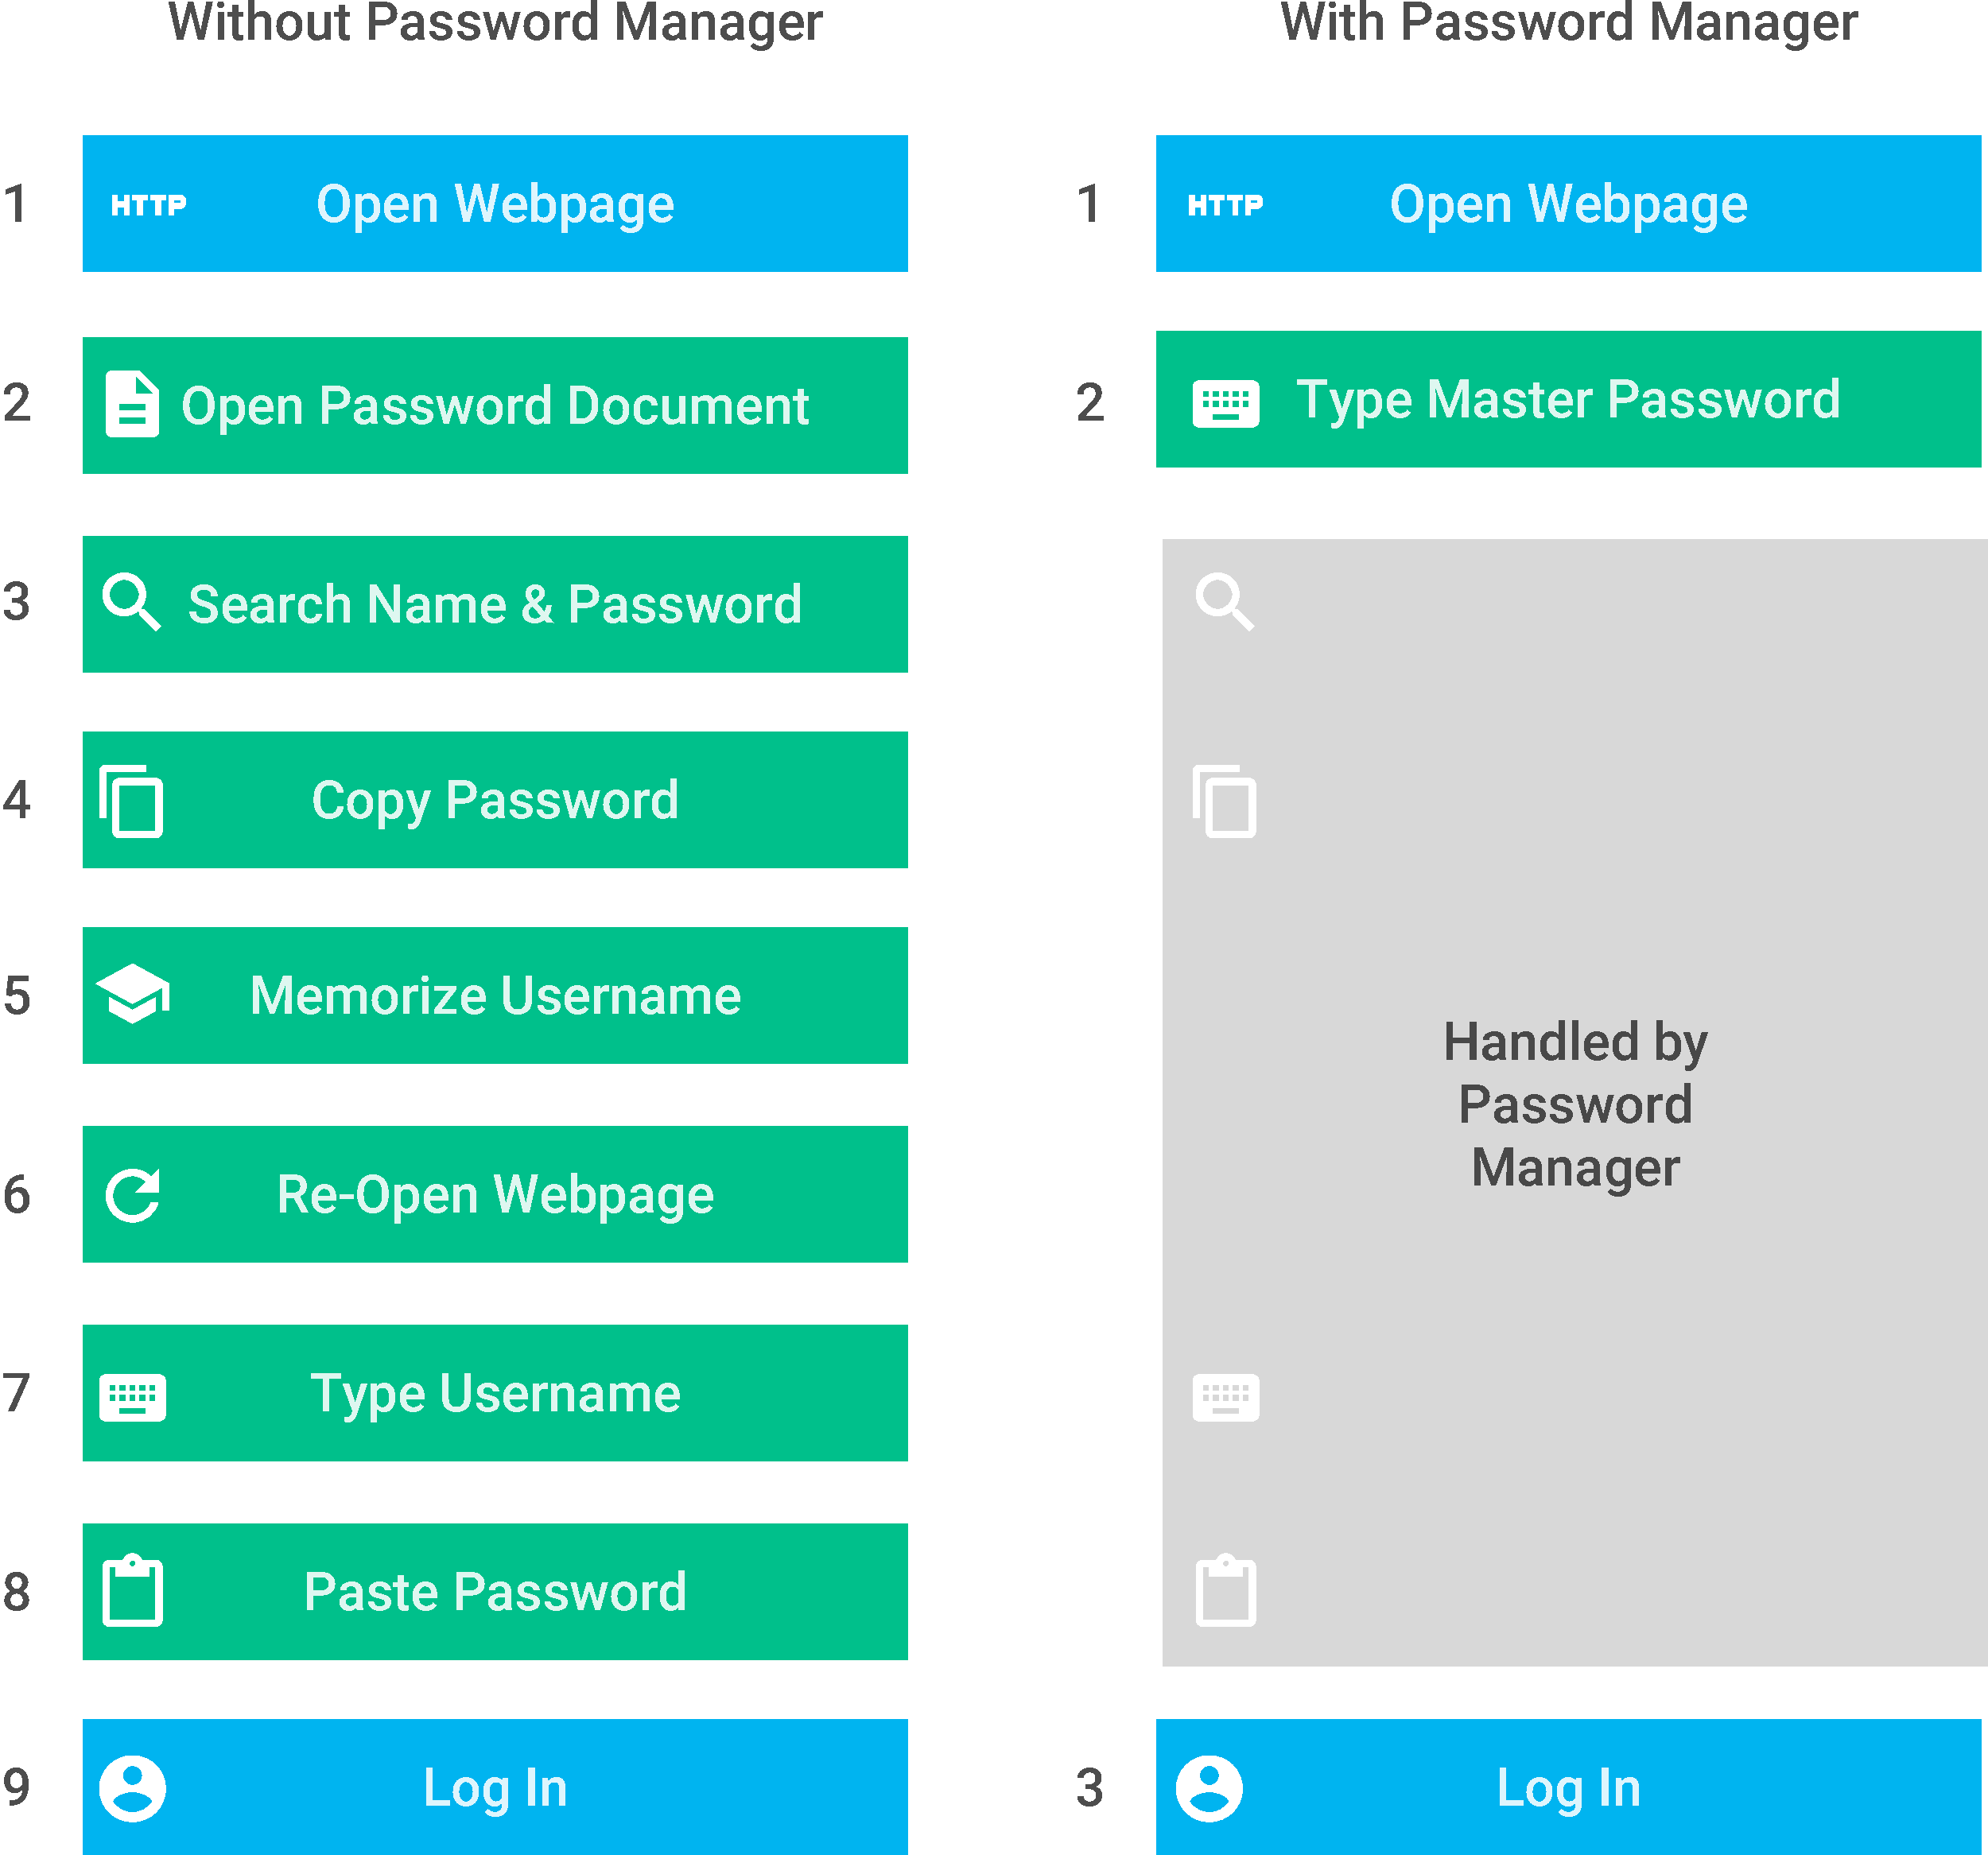
\includegraphics[width=0.6\linewidth]{mm_pwm/pwm-goms-comparison}
	\caption{\label{fig:mm_pwm:pwm-goms-comparison} Visualizing users' previous behavior might help communicate how the password manager can simplify authentication tasks. This can create a better mental model of their workings.}
\end{figure}

%- trust was not an issue because they were generally unaware of the existence of PWM.

\subsection{Increasing Sense of Agency}
While automation simplifies processes and thus improves usability, staying in control of security-related interactions is important to users. \textit{Novices} were confident in their current behavior. \textit{Actives} had realized that their past behavior was sub-optimal, but they had gained confidence to create passwords and handle authentication for their most important accounts on their own. As a consequence, a password manager needs to stay flexible enough to respect user preferences for different account \textit{categories}, e.g. unimportant vs. important accounts. At the same time, reassuring users that their decision to handle such situations on their own is reasonable and can inspire trust in the system. A PWM could automatically detect when it is appropriate to offer help. Current managers only provide the opportunity to decide whether the password should be saved, maybe saved later, or never be saved for a particular site. Such decisions can be automated once enough training data has been provided by the user.

\subsection{Leveraging Context}
Context factors can be leveraged by PWMs to adapt to different situations. For example, usage-context informs future interactions. If the user sets up the system at work, this is an indicator about how passwords are going to be categorized, how often they will be reset, and how likely they are going to be shared with others. Adapting the interface to such scenarios can simplify interactions and forming mental models of the benefits. Moreover, automated generation of passwords is also context-dependent. As we have shown in chapter \ref{chap:policies_reuse}, password policies in the wild impose varying restrictions on the use of characters. To avoid user frustration arising from rejected passwords, e.g. because they contain forbidden characters, the generator can ensure the random password meets the website's composition policy. 

%- onboarding process: usage at home or at work / customized/adaptive onboarding
%- better embedding in sign-up forms 
%- automatic password generation should consider password policy. --> see chapter \ref{chap:policies_reuse}

\subsection{Customization and Personalization}
It is evident that current third-party and browser-built-in password managers work fundamentally differently to how users normally cope with passwords. Our participants reused passwords with different strategies and relied on digital documents, paper notes, and highly individual password creation or memorization techniques. Beside the document-metaphor discussed above, the other strategies are not reproduced by password managers. However, a general philosophy in user-centered design is the aim to ``fix the system'' rather than to ``fix the user''. Therefore, the system should leverage existing strategies. For instance, it could let the user specify a creation technique: if they usually modify a base-password depending on the context, the PWM could offer to generate passwords like this in future scenarios, i.e., automate the modification strategy. While this approach would not necessarily improve security, it could save the user time and remove critical pain points. Besides, the user stays independent of the tool, because they can reproduce their personal system and authenticate on other devices even without the support. 

%- current pwms do not support many behaviors that users still do: reuse, word documents, paper notes, individual creation and memorization techniques, reuse strategies. 
% - maybe target persona elliot elis

%\subsection{Limitations}

\section{Conclusion}
We explored the mental models of authentication tasks and password managers with a qualitative approach. Both participants experienced with password managers and inexperienced novices shared their insights, attitudes and behaviors during short interviews. Fourteen interviewees provided us detailed descriptions of their password selection and coping strategies, and how they make sense of supporting tools. 
% how does this change the world?
We contribute evidence that (a) individual coping strategies persist even after adopting a password manager for important accounts, (b) work environments serve as onboarding triggers even for private use, and (c) novices were mostly unaware of functionality and the ramifications of adopting password managers. 
% larger vision.
These findings show that the value proposition should be communicated concisely and compare the benefits against inefficient password practices. At the same time, new solutions should respect highly individual coping strategies to better match user behavior. Ultimately, this could increase adoption, and more importantly, retention rates. 


\noindent
\fbox{
	\hspace{1cm}
	\parbox[c][12cm]{0.7\linewidth}{
		\section*{Take Aways}
		\begin{itemize}[leftmargin=*]
%			\item The system architecture of a password manager is difficult to frame visually both for people who have never used one, and also for users. Active users created more visually rich sketches, but this was likely due to their professional background. 
			\item Password managers appear to be a ``black box'' for people who have never used one. They suspect that such tools are a slightly more secure version of text files to write down lists of username-password-combinations.
			\item The mental model of password authentication and managers is mostly divided into the mental spaces ``Select password'', ``Log in'', and ``Organize''. There seem to be discrepancies between current user behavior and current password managers. 
			\item Making password managers adapt to context and individuals seems a promising direction for future systems. 
		\end{itemize}
	}
	\hspace{1cm}
}




